\documentclass[a4paper,12pt]{report}

\usepackage[utf8]{inputenc}
\usepackage[french]{babel}
\usepackage[T1]{fontenc}
%\usepackage[scaled]{helvet} % police
\usepackage{lmodern}
\usepackage{layout}
\usepackage[top=2cm, bottom=1.5cm, left=2cm, right=2cm]{geometry}
\usepackage{setspace}
\usepackage{verbatim}
\usepackage{moreverb}
\usepackage{listings}
\usepackage{graphicx}
\usepackage{shorttoc}
\usepackage{xcolor}
\usepackage{currfile}
\usepackage{hyperref}
\usepackage{array}

\setcounter{topnumber}{4}
\setcounter{bottomnumber}{4}
\setcounter{totalnumber}{10}
\renewcommand{\textfraction}{0.15}
\renewcommand{\topfraction}{0.85}
\renewcommand{\bottomfraction}{0.70}
\renewcommand{\floatpagefraction}{0.66}

%\include{chapterStyle}

\makeatletter
\def\thickhrulefill{\leavevmode \leaders \hrule height 1ex \hfill \kern \z@}
\def\@makechapterhead#1{%
  \vspace*{10\p@}%
  {\parindent \z@ \raggedleft \reset@font
            \scshape \@chapapp{} \thechapter
        \par\nobreak
        \interlinepenalty\@M
    \Huge \bfseries #1\par\nobreak
    %\vspace*{1\p@}%
    \hrulefill
    \par\nobreak
    \vskip 20\p@
  }}
\def\@makeschapterhead#1{%
  \vspace*{10\p@}%
  {\parindent \z@ \raggedleft \reset@font
            \scshape \vphantom{\@chapapp{} \thechapter}
        \par\nobreak
        \interlinepenalty\@M
    \Huge \bfseries #1\par\nobreak
    %\vspace*{1\p@}%
    \hrulefill
    \par\nobreak
    \vskip 20\p@
  }}

\renewcommand\thesection{\arabic{section}}
%\renewcommand*\familydefault{\sfdefault} %% Only if the base font of the document is to be sans serif


% Redéfinition de commandes

% Pour avoir les noms de chapitre en 1.1.3 etc...
\renewcommand\thesection{\arabic{chapter}.\arabic{section}}

% Désactiver les alinéas automatiques
%\parindent=0cm


% Création du glossaire

\setcounter{tocdepth}{4}

\begin{document}
  \begin{onehalfspace}

  % Page de garde
    \begin{titlepage}
      \begin{center}
        Sébastien Corbin et François-Guillaume Ribreau\\
        CSII 3\ieme année\\
        Le 21 Septembre 2011\\
      \end{center}
      \hrulefill
      \vspace{7cm}
      \begin{center}
        \LARGE \textbf{Dossier de spécifications}\\
        \vspace{3cm}
        \normalsize Génie Logiciel Embarqué
      \end{center}

      \vspace{9,5cm}

      \begin{center}
      \line(1,0){250}
      \end{center}

      \begin{center}
      \tiny{\currfilename}
      \end{center}
  
   \setcounter{page}{0}
    \end{titlepage}
    \clearpage

\chapter{But du document}
Le but de ce document est de lister toutes les fonctionnalités du projet GeoBBS ainsi que de donner un aperçu des interfaces et des interactions la composant. Ce document fournit aussi une description des utilisateurs et leur rôle dans le logiciel.

\chapter{Diagramme de cas d'utilisation}

\begin{center}
  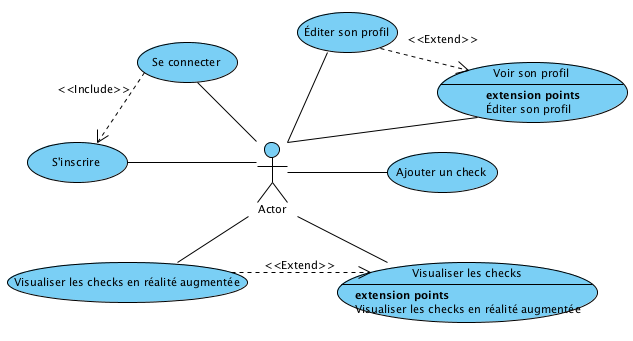
\includegraphics[width=17cm]{img/diag_cas_utilisation.png}
\end{center}


\chapter{Description globale}

\subsection{Environnement} % (fold)
\label{sub:environnement}
L’application est hébergée sur le serveur internet de la société GEOBBS CORP. Et est accessible depuis l’extérieur via l'application mobile.

% subsection environnement (end)

\subsection{Profils des utilisateurs} % (fold)
\label{sub:profils_des_utilisateurs}

GeoBBS accepte deux types d’utilisateurs, les visiteurs et les membres.

\subsubsection{Les visiteurs}
Toute personne qui arrive sur le site (ou l'application) pour la première fois et qui ne possède pas de compte ou n’est pas connecté est appelée visiteur.

\subsubsection{Les membres}
Un membre est une personne qui s’est identifiée auprès du site (ou de l'application mobile). Elle est distinguée des autres membres par un identifiant unique et peux utiliser l’intégralité des services qu’offre GeoBBS.


\chapter{Spécifications générales} % (fold)
\label{cha:sp_cifications_g_n_rales}

\subsection{Description des services attendus}

Les services attendus sont répartis dans les différents modules de l’application. Ces modules sont accessibles ou non en fonction du type d’utilisateur, visiteur ou membre.

Les visiteurs ont uniquement accès au formulaire de création de compte et au formulaire de connexion. Aucun autre écran n’est accessible au grand public.

Les membres peuvent agir sur les 4 grands modules :
\begin{description}
  \item[Near] répertories les membres proches géographiquement de l'utilisateur actuel
  \item[Check] permet au membre de "checker" c'est à dire informer proactivement GeoBBS de sa position en y ajoutant s'il le souhaite une description et une image (ou vidéo)
  \item[AR] Affiche en réalité augmenté les points d'intérêts autour de l'utilisateur
  \item[Profil] permet à l'utilisateur d'éditer son profil
\end{description}

\subsection{Approche utilisée dans ce document} % (fold)
\label{sub:approche_utilis_e_dans_ce_document}
Plutôt que de disperser les spécifications (diagramme de cas d’utilisation, diagramme de classe, diagramme de séquence, maquettes) d’un même module à diverses endroits du document. La spécification par composant a été préférée. Elle permet une lecture plus aisée et rapide de l’intégralité du fonctionnement d’un composant d’un module.
% subsection approche_utilis_e_dans_ce_document (end)

\subsection{Description générale des fonctions} % (fold)
\label{sub:description_g_n_rale_des_fonctions}

\chapter{Cas d'utilisation}
Un visiteur peut effectuer 2 actions, s’inscrire et se connecter.

\subsubsection{Cas d'utilisation: le visiteur s'inscrit} % (fold)

%%%%%%%%%%%%
\begin{tabular}{|p{3cm}|p{12,5cm}|}
\hline %%

\textbf{But} &
Enregistrer les informations du visiteur en base 
\\ \hline %%

\textbf{Résumé} &
Le visiteur s'inscrit au service via l'application mobile
\\ \hline %%

\textbf{Acteurs} &
Visiteur (acteur principal)
\\ \hline %%

\multicolumn{2}{|c|}{\textbf{Description des enchaînements}} \\ \hline %%

\textbf{Pré-conditions} &
Le site est accessible, la base de données est disponible, le visiteur est sur le site
\\ \hline %%

\textbf{Enchaînements nominaux} &
Évènement déclencheur : Lorsque le visiteur souhaite se créer un compte
\\ \hline %%

\textbf{Enchaînements alternatifs} &
    \begin{description}
      \item[Alternative 1]: Le visiteur souhaite se connecte via son compte Facebook, Twitter.
    \end{description}
\\ \hline %%

\textbf{Enchaînements d'erreurs} &
  \begin{description}
    \item[Exception 1]: Les informations obligatoires ne sont pas toutes saisies
    \begin{itemize}
      \item Afficher un message d’erreur récapitulant les champs restant à saisir
    \end{itemize}
    \item[Exception 2]: Certaines informations saisies sont incorrectes (Email, nom d’utilisateur, code postal)
    \item[Exception 3]: Le nom d’utilisateur est déjà présent en BDD
    \begin{itemize}
      \item Afficher un message d’erreur : « Ce nom d’utilisateur est déjà présent en BDD, veuillez en choisir un autre »
    \end{itemize}
  \end{description}
\\ \hline %%

\textbf{Post-conditions} &
\\ \hline %%

\end{tabular}
%%%%%%%%%%%%


\subsubsection{Cas d'utilisation : le visiteur se connecte} % (fold)

%%%%%%%%%%%%
\begin{tabular}{|p{3cm}|p{12,5cm}|}
\hline %%

\textbf{But} &
Récupérer les informations du visiteur en base 
\\ \hline %%

\textbf{Résumé} &
\\ \hline %%

\textbf{Acteurs} &
\begin{itemize}
  \item Visiteur (acteur principal)
\end{itemize} 
\\ \hline %%

\multicolumn{2}{|c|}{\textbf{Description des enchaînements}}
\\ \hline %%

\textbf{Pré-conditions} &
    \begin{itemize}
      \item Le serveur est accessible, la base de données est disponible    
    \end{itemize}
\\ \hline %%

\textbf{Enchaînements nominaux} &
    \begin{itemize}
      \item Évènement déclencheur : Lorsque le visiteur souhaite se créer un compte
    \end{itemize}
\\ \hline %%

\textbf{Enchaînements alternatifs} &
    \begin{description}
      \item[Alternative 1]: Le visiteur souhaite s’inscrire via son compte Facebook, Twitter. TODO:
    \end{description}
\\ \hline %%

\textbf{Enchaînements d'erreurs} &
  \begin{description}
    \item[Exception 1]: Les informations obligatoires ne sont pas toutes saisies
    \begin{itemize}
      \item Afficher un message d’erreur récapitulant les champs restant à saisir
    \end{itemize}
    \item[Exception 2]: Certaines informations saisies sont incorrectes (Email, nom d’utilisateur, code postal)
    \item[Exception 3]: Le nom d’utilisateur est déjà présent en BDD
    \begin{itemize}
      \item Afficher un message d’erreur : « Ce nom d’utilisateur est déjà présent en BDD, veuillez en choisir un autre »
    \end{itemize}
  \end{description}
\\ \hline %%

\textbf{Post-conditions} &
\\ \hline %%

\end{tabular}
%%%%%%%%%%%%

\subsubsection{Cas d'utilisation : le visiteur visualise les checks} % (fold)

%%%%%%%%%%%%
\begin{tabular}{|p{3cm}|p{12,5cm}|}
\hline %%

\textbf{But} &
Visualiser les checks à proximité
\\ \hline %%

\textbf{Acteurs} &
Visiteur (acteur principal)
\\ \hline %%

\multicolumn{2}{|c|}{\textbf{Description des enchaînements}}
\\ \hline %%

\textbf{Pré-conditions} &
    \begin{itemize}
      \item Le site est accessible
      \item La base de données est disponible
      \item Le visiteur a lancé l'application et est connecté
    \end{itemize}
\\ \hline %%

\textbf{Enchaînements nominaux} &
Évènement déclencheur : Lorsque le visiteur souhaite visualiser les checks
\\ \hline %%

\textbf{Enchaînements alternatifs} &
\\ \hline %%

\textbf{Enchaînements d'erreurs} &
  \begin{description}
    \item[Exception 1]: La connexion au réseau est indisponible
    \begin{itemize}
      \item Afficher un message d’erreur à l'utilisateur
    \end{itemize}
  \end{description}
\\ \hline %%

\textbf{Post-conditions} &
\\ \hline %%

\end{tabular}
%%%%%%%%%%%%

\subsubsection{Cas d'utilisation : Le visiteur ajoute un check}
%%%%%%%%%%%%
\begin{tabular}{|p{3cm}|p{12,5cm}|}
\hline %%

\textbf{But} &
Envoyer un check avec un message et une position associée
\\ \hline %%

\textbf{Résumé} &
Le visiteur tape un message puis l'envoie avec sa position actuelle
\\ \hline %%

\textbf{Acteurs} &
Visiteur (acteur principal)
\\ \hline %%

\multicolumn{2}{|c|}{\textbf{Description des enchaînements}}
\\ \hline %%

\textbf{Pré-conditions} &
    \begin{itemize}
      \item Le site est accessible
      \item La base de données est disponible
      \item Le visiteur a lancé l'application et est connecté
    \end{itemize}
\\ \hline %%

\textbf{Enchaînements nominaux} &
  Évènement déclencheur : Lorsque le visiteur souhaite poster un check
\\ \hline %%

\textbf{Enchaînements alternatifs} &
\\ \hline %%

\textbf{Enchaînements d'erreurs} &
  \begin{description}
    \item[Exception 1]: La position de l'utilisateur ne peut être déterminée
    \begin{itemize}
      \item Afficher un message d’erreur informant l'utilisateur
    \end{itemize}
    \item[Exception 2]: Le message n'est pas renseigné
    \begin{itemize}
      \item Afficher un message d’erreur récapitulant les champs restant à saisir
    \end{itemize}
    \item[Exception 3]: La connexion au réseau est indisponible
    \begin{itemize}
      \item Afficher un message d’erreur informant l'utilisateur
    \end{itemize}
  \end{description}
\\ \hline %%

\textbf{Post-conditions} &
\\ \hline %%

\end{tabular}
%%%%%%%%%%%%


\subsubsection{Cas d'utilisation : Le visiteur visualise son profil}
%%%%%%%%%%%%
\begin{tabular}{|p{3cm}|p{12,5cm}|}
\hline %%

\textbf{But} &
Visualiser le profil de l'utilisateur
\\ \hline %%

\textbf{Acteurs} &
Visiteur (acteur principal)
\\ \hline %%

\multicolumn{2}{|c|}{\textbf{Description des enchaînements}}
\\ \hline %%

\textbf{Pré-conditions} &
    \begin{itemize}
      \item Le site est accessible
      \item La base de données est disponible
      \item Le visiteur a lancé l'application et est connecté
    \end{itemize}
\\ \hline %%

\textbf{Enchaînements nominaux} &
  Évènement déclencheur : Lorsque le visiteur souhaite accéder à son profil
\\ \hline %%

\textbf{Enchaînements alternatifs} &
\\ \hline %%

\textbf{Enchaînements d'erreurs} &
  \begin{description}
    \item[Exception 1]: La connexion au réseau est indisponible
    \begin{itemize}
      \item Afficher un message d’erreur informant l'utilisateur
    \end{itemize}
  \end{description}
\\ \hline %%

\textbf{Post-conditions} &
\\ \hline %%

\end{tabular}
%%%%%%%%%%%%

\paragraph*{}
Voici une liste d'autres cas d'utilisation relativement similaires qui seront implicitement traités :
\begin{itemize}
  \item Visualiser les checks en réalité augmentée
  \item Modifier son profil
  \item Consulter le profil d'un autre utilisateur
\end{itemize}

\chapter{Ecrans} % (fold)
\label{cha:ecrans_suppl_mentaires}
\begin{center}

\end{center}

\chapter{Diagramme de classes} % (fold)
\label{cha:diagramme_de_classes}

L'application serveur et l'application mobile étant des prototypes développés suivant le paradigme fonctionnel, ils n'utilisent aucun classe. Il n'y a donc pas de diagramme de classe dans ce document. Cependant les spécifications futures (post-prototype) inclueront classes et un diagramme de classe devra donc être présent.

\chapter{Spécifications technologiques et opératoires}

% chapter diagramme_de_classes (end)

% chapter ecrans_suppl_mentaires (end)
% subsection description_g_n_rale_des_fonctions (end)
\section{Matériel}
\subsection{Description}
L'iPhone  est une famille de smartphones conçue et commercialisée par Apple Inc. depuis 2007. Les modèles, dont l'interface utilisateur a été conçue avec le multi-touch, disposent d'un appareil photo, d'une fonction baladeur numérique, d'un client Internet (pour naviguer sur le Web ou consulter son courrier électronique), et de fonctions basiques telles que les SMS/MMS (messages texte et multimédia) ; mais disposent aussi de la messagerie vocale visuelle et de l'App Store, qui permet de télécharger des applications, allant des jeux aux réseaux sociaux, en passant par les GPS, la télévision, la presse électronique ou encore les bandes-dessinées. Au mois de mai 2010, on compte plus de 225 000 applications.

\subsection{Spécifications}
Les spécifications suivantes sont relatives à l'iPhone 4 (génération Juin 2010)
  \begin{description}
  \item[Système d'exploitation] iOS 4.3.5 (build 8L1, sortie le 25 juillet 2011)
  \item[Alimentation] Batterie lithium-polymère
  \item[Processeur] Puce apple A4 1 GHz
  \item[Stockage]  16/32 Go de mémoire flash
  \item[Mémoire] 512 Mio de DRAM
  \item[Écran] Écran multi-touch de 3,5 pouces
  \item[Résolution] 960 x 640 px (326 ppp)
  \item[Carte graphique]  PowerVR SGX 535 GPU
  \item[Caméra] \emph{Arrière} : 5 mégapixels, vidéo 720p avec Flash LED / \emph{Avant} : VGA
  \end{description}

\section{Le système d'exploitation iOS}
iOS, (anciennement iPhone OS), est le système d'exploitation mobile développé par Apple pour l'iPhone, l'iPod touch, et l'iPad. Il est dérivé de Mac OS X dont il partage les fondations (le kernel hybride XNU basé sur le micro-noyau Mach, les services Unix et Cocoa, etc.). iOS comporte quatre couches d'abstraction, similaires à celles de Mac OS X : une couche « Core OS », une couche « Core Services », une couche « Media » et une couche « Cocoa ». Le système d'exploitation occupe moins d'un demi-gigaoctet (Go) de la capacité mémoire totale de l'appareil.

\section{L'environnement de développement}
Le kit de développement, disponible uniquement pour Mac OS X, propose les outils nécessaires à la création d'une application pouvant tourner sous iOS. Si son téléchargement et son utilisation sont gratuits, la publication de telles applications requiert d'adhérer au programme des développeurs Apple, pour la somme de 99\$ par an. Il n'en demeure pas moins que cette offre peut s'avérer intéressante pour bon nombre de développeurs, étant donnée la taille du marché créé par iOS.
En plus d'offrir aux développeurs exactement les mêmes API que celles d'Apple, le SDK contient de nombreux outils facilitant le développement et le test d'applications pour iOS.

\subsection{Outils de développement}
La plupart des outils de développement du SDK étaient déjà présents dans Mac OS avant son arrivée. Cependant, ils gèrent désormais l'utilisation de l'iPhone, en tant que plate-forme de développement :
\begin{description}
\item[Xcode] Environnement de Développement Intégré par défaut sur Mac OS X. Il permet l'écriture, la gestion et la compilation de projets de développement, écrits notamment en Objective-C. L'iPhone SDK y ajoute les librairies de développement pour iOS. Il est donc possible pour le développeur de créer des projets d'applications pour ce système. Pour tester l'application, deux possibilités existent : le développeur peut brancher un iPhone ou iPod Touch à son ordinateur Mac, puis y lancer l'application comme test, ou lancer l'application en test dans iPhone Simulator.
\item[Interface Builder] permet de construire une interface pour Cocoa Touch manuellement, à l'aide de glisser-déposer. Il permet également de traduire facilement une application dans plusieurs langues. De plus, il permet de gérer visuellement le schéma Modèle-Vue-Contrôleur, en connectant des éléments d'une interface à un code écrit pour eux au préalable, à l'aide d'un glisser-déposer. Finalement, le fichier d'interface ainsi créé est ajouté au projet Xcode.
Instruments est un outil de monitoring informatique. Il permet, une fois l'application lancée sur un iPhone ou iPod Touch branché à l'ordinateur, d'observer en temps réel ses performances au niveau du processeur, mais également, par exemple, du moteur graphique ou de l'accéléromètre. Par ailleurs, il est également possible de surveiller les performances système dans iPhone Simulator.
\item[iPhone Simulator] simule de manière logicielle un iPhone virtuel, qui peut exécuter des applications directement sur l'ordinateur. Les mouvements Multitouch sont alors reproduits manuellement à la souris par l'utilisateur, et il est possible de faire pivoter le simulateur grâce à des raccourcis clavier. Par ailleurs, l'utilisateur est en mesure de choisir quelle version du firmware il désire utiliser.
\end{description}

\chapter{Architecture serveur}

Le serveur est développé en NodeJS, il interagit avec le reste de la plateforme (client mobile) via le protocole HTTP sur le port 3000. L'architecture est de type REST (basée sur la thèse Roy Fielding cf. documents de références). Chaque ressource est identifiée par une URI (Uniform Ressource Indentifier).

\newline
L'adresse du serveur et le port sont défini directement dans le code de l'application.

Seront décrit dans la suite de ce document les différents points d'entrée

\section{Points d'entrée}
\begin{description}
  \item[POST /check/create/]:

    \begin{description}
      \item[Description] Ajoute un check
      \item[Paramètres]:

        \begin{description}
          \item[userId (string)] Id de l'utilisateur
          \item[lat (float)] Latitude
          \item[lon (float)] Longitude
          \item[description (string)] (optionel) Description du check
          \item[imgUrl (string)] (optionel) Url de l'image à lier
        \end{description}
    \end{description}

  \item[GET /check/list/]:

    \begin{description}
      \item[Description] Retourne la liste des checks aux alentours de \lstinline{lat},\lstinline{lon}.

      \item[Paramètres]:
        \begin{description}
          \item[userId (string)] Id de l'utilisateur
          \item[lat (float)] Latitude
          \item[lon (float)] Longitude
          \item[distance (entier)] (optionel) Distance maximum par rapport à \lstinline{lat},\lstinline{lon}.
          \item[count (entier)] (optionel) Nombre maximum de données à retourner
        \end{description}
    \end{description}

  \item[GET /user/profil/]:

    \begin{description}
      \item[Description] Affiche une page HTML d'édition du profil et des préférences de l'utilisateur.

      \item[Paramètres]:
        \begin{description}
          \item[userId (string)] Id de l'utilisateur
        \end{description}
    \end{description}

\end{description}

\chapter{Base de données}

L'administration de la base de donnée se fera par l'utilisateur via \lstinline{RockMongo} ou \lstinline{MongoHub}.

\paragraph*{}
Collections en BDD :
\begin{description}
  \item[users] collection des utilisateurs
  \item[checks] collection des checks
\end{description}


\paragraph*{}
Ajout d'une première entité dans Checks :
\begin{description}
  \item[loc] \lstinline{[1,1]}
  \item[\_userId] \lstinline{ObjectId("4e7e0614bd99e29380000000")}
  \item[date] \lstinline{new Date()}
  \item[description] \lstinline{test}
  \item[User] \lstinline{ login: FG }
\end{description}

\paragraph*{}
Ajout d'une première entité dans Users :
\begin{description}
  \item[login] \lstinline{FG}
  \item[password] \lstinline{"098f6bcd4621d373cade4e832627b4f6"} ("test" en MD5)
  \item[checks] \lstinline{[ObjectId("4e7e0614bd99e09890000000")]}
\end{description}

\paragraph*{}
Ajout d'un index sur les checks via le CLI \lstinline{$mongo}:
\begin{lstlisting}[float=htb, language=bash, frame=lines, caption={Commandes à entrer dans le CLI mongo}, label={code:cliMongo}]
> use geobbs
> db.checks.ensureIndex({ loc : "2d" })
\end{lstlisting}

\chapter{Délimitation de l'application}
TODO: expliquer que nous sommes parti sur un prototype et que nous ne réaliserons pas l'intégralité de la plateforme pour des raisons de temps.

% \chapter*{Ce qu'il faut traiter}
% Intro
%   Les os de l'embarqué
%   ->(liste et ce qu'il font chacun)
%
%   Notion d'entrée/sortie
%
%   Les Env. de dev (avec particularité du remote debugging)
%
%   Résumé des différentes méthodes (agile, xp etc..., tdd etc...)
%
% Projet
%   -> Equipe
%   -> Cahier des charges
%
% Choix de la méthodo:
%   -> Méthode Agile
%   -> + TDD
%
% Languages:
% Objective-C / JavaScript
%
% Libraries:
% ExpressJS (serveur http)
% Mongoose http://mongoosejs.com/ (mongodb)
%
% La sécuration est faites par oAuth

% \chapter*{Matériel existant}
% iPhone

% MacBookPro 13 et 15 pouces

% \chapter*{Analyse des librairies}

% \href{http://developer.apple.com/library/ios/documentation/iPhone/Conceptual/iPhoneOSProgrammingGuide/index.html}{Guide de programmation iOs}

% Géolocalisation:

% \href{http://developer.apple.com/library/ios/documentation/UserExperience/Conceptual/LocationAwarenessPG/Introduction/Introduction.html}{Introduction au développement relatif à la géolocalisation}


  \end{onehalfspace}
\end{document}
